
\section{Multivariate linear models: HE plots}\label{sec:mlm}

%\TODO{
%\begin{itemize*}
%\item H ellipse: data ellipse of fitted values; E ellipse: data ellipse of residuals [done]
%\item Visual tests of significance: Radii, volumes, etc
%\item Linear hypotheses: Geometries of contrasts and sums of effects
%\item Canonical projections; ellipses in data space and canonical space
%\end{itemize*}
%}

Multivariate linear models (\MLM{}s) have a special affinity with ellipsoids and elliptical geometry,
as described in this section.  To set the stage and establish notation, we consider
the \MLM\ (e.g., \citet{Timm:75}) given by
the equation $\mat{Y}=\mat{XB}+\mat{U}$, where $\mat{Y}$ is an $%
n\times p$ matrix of responses in which each column represents a distinct
response variable; $\mat{X}$ is the  $n\times q$ model matrix of full
column rank for the regressors; $\mat{\Beta}$ is the $q \times p$ matrix
of regression coefficients or model parameters; and $\mat{U}$ is the $n \times p$
matrix of errors,
with $\textrm{vec}(\mat{U}) \sim \mathcal{N}_p ( \mat{0}, \mat{I}_n \otimes \mat{\Sigma} )$,
where $\otimes$ is the Kronecker product.

A convenient feature of the \MLM\ for general multivariate responses is that
\emph{all} tests of linear hypotheses (for null effects) can be represented in the form of a general
linear test,
\begin{equation}\label{eq:mglt}
H_0 : \sizedmat{L}{h \times q}
\sizedmat{\Beta}{q \times p} =
\sizedmat{0}{h \times p}
\comma
\end{equation}
where $\mat{L}$ is a rank $h \leq q$ matrix of constants whose rows specify
$h$ linear combinations or contrasts
of the parameters to be tested simultaneously
by a multivariate test.

For \emph{any} such hypothesis of the form given in \eqref{eq:mglt}, the analogs of the univariate
sums of squares for hypothesis ($\mathrm{SS}_H$) and error ($\mathrm{SS}_E$)
are the $p \times p$  sum of squares and crossproducts (SSP) matrices given by:
\begin{equation} \label{eq:hmat}
\mat{H}  \equiv \mat{SSP}_H =
 (\mat{L} \widehat{\mat{B}})\trans \,
 [\mat{L} (\mat{X}\trans \mat{X} )^{-} \mat{L}\trans]^{-1} \,
 (\mat{L} \widehat{\mat{B}})
 \comma
\end{equation}
and
\begin{equation} \label{eq:emat}
\mat{E}  \equiv \mat{SSP}_E =
 \mat{Y}\trans \mat{Y} -
 \widehat{\mat{B}}\trans (\mat{X}\trans \mat{X}) \widehat{\mat{B}}
 =
  \widehat{\mat{U}}\trans  \widehat{\mat{U}}
 \comma
\end{equation}
where $\widehat{\mat{U}} = \mat{Y} - \mat{X} \widehat{\mat{B}}$ is the matrix of residuals.
Multivariate test statistics (Wilks's $\Lambda$, Pillai trace, Hotelling-Lawley trace, Roy's maximum root)
for testing \eqref{eq:mglt} are based on the $s = \min(p, h)$ non-zero latent roots
$\lambda_{1}>\lambda_{2}>\cdots>\lambda_{s}$ of
the matrix \mat{H} relative to the matrix \mat{E}, that is,
the values of $\lambda$ for which $
\detbracket{\mat{H}-\lambda\mat{E}}=0$, or equivalently
the latent roots $\rho_i$ for which $\det{\mat{H} - \rho (\mat{H}+\mat{E})}=0$.
The details are shown in \tabref{tab:criteria}.
% but note that $\rho_i = \lambda_i / (1+\lambda_i)$ 
These measures
attempt to capture how ``large'' $\mat{H}$ is, relative to
$\mat{E}$ in $s$ dimensions, and correspond to various ``means'' as we described earlier.
All of these statistics have transformations to $F$ statistics
giving either exact or approximate null-hypothesis $F$ distributions.
The corresponding latent vectors provide a
set of $s$ orthogonal linear combinations of the responses that produce
maximal univariate $F$ statistics for the hypothesis in \eqref{eq:mglt};
we refer to these as the \emph{canonical discriminant} dimensions.


\begin{table}[htb]
\renewcommand{\arraystretch}{1.6}
\caption{Multivariate test statistics as functions of the eigenvalues $\lambda_i$ solving $\det{\mat{H} - \lambda \mat{E}}=0$
or eigenvalues $\rho_i$ solving  $\detbracket{\mat{H} - \rho (\mat{H}+\mat{E})}=0$.
}\label{tab:criteria}
\begin{center}
\begin{tabular}{|l|l|l|l|}
  \hline
  % after \\: \hline or \cline{col1-col2} \cline{col3-col4} ...
  Criterion & Formula & ``mean'' of $\rho$ & Partial $\eta^2$   \\
  \hline
  Wilks's $\Lambda$ & $\Lambda = \prod^s_i \frac{1}{1+\lambda_i} = \prod^s_i (1-\rho_i)$ & geometric & $\eta^2 = 1-\Lambda^{1/s}$   \\
  Pillai trace & $V = \sum^s_i \frac{\lambda_i}{1+\lambda_i} = \sum^s_i \rho_i$ & arithmetic & $\eta^2 = \frac{V}{s} $   \\
  Hotelling-Lawley trace & $H = \sum^s_i \lambda_i = \sum^s_i \frac{\rho_i}{1-\rho_i} $ & harmonic & $\eta^2 = \frac{H}{H+s}$   \\
  Roy maximum root & $R = \lambda_1 = \frac{\rho_1}{1-\rho_1}$  & supremum & $ \eta^2 = \frac{\lambda_1}{1+\lambda_1} = \rho_1$   \\
  \hline
\end{tabular}
\end{center}
\end{table}
%\end{document}


\subsection{Hypothesis-Error (HE) plots}

The essential idea behind HE plots is that any multivariate hypothesis
test \eqref{eq:mglt} can be represented visually by ellipses (or ellipsoids beyond 2D) that express
the size  of covariation against a multivariate null hypothesis
($\mat{H}$) relative to error covariation ($\mat{E}$).
The multivariate tests, based on the latent roots of $\mat{H} \mat{E}^{-1}$,
are thus translated directly to the sizes of the \mat{H} ellipses for
various hypotheses, relative to the size of the \mat{E} ellipse.
Moreover, the shape and orientation of these ellipses show something more---the
directions (linear combinations of the responses) that lead to
various effect sizes and significance.

\begin{figure}[htb]
  \centering
  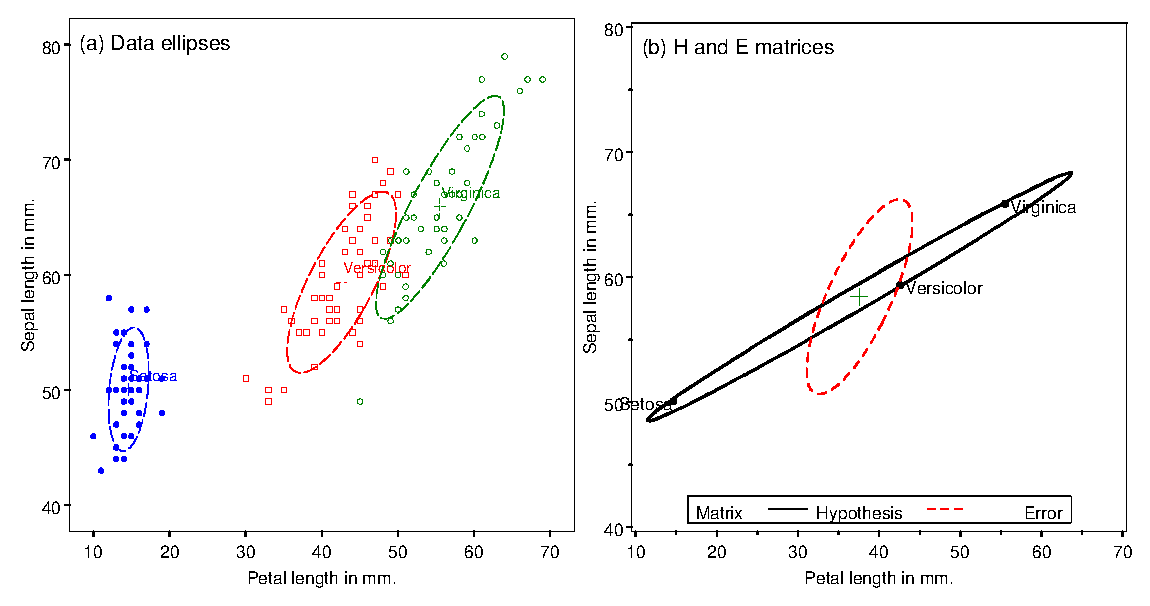
\includegraphics[width=.9\textwidth,clip]{fig/heplot3a}
  \caption{(a) Data ellipses and (b) corresponding HE plot for sepal length and petal length in the iris dataset.
  	The \mat{H} ellipse is the data ellipse of the fitted values defined by the group means, $\bar{\vec{y}}_{i \cdot}$
  	The \mat{E} ellipse is the data ellipse of the residuals, $(\vec{y}_{ij} - \bar{\vec{y}}_{i \cdot})$.
  	Using evidence (``significance'') scaling of the \mat{H} ellipse, the plot has the property that
  	the multivariate test for a given hypothesis is significant by Roy's largest-root test \emph{iff}
  	the \mat{H} ellipse protrudes anywhere outside the \mat{E} ellipse.}%
  \label{fig:heplot3a}
\end{figure}

\figref{fig:heplot3a} illustrates this idea for two variables from the iris dataset.
Panel (a) shows the data ellipses for sepal length and petal length, equivalent to
the corresponding plot in \figref{fig:scatirisd1}. Panel (b) shows the HE plot for these
variables from the one-way MANOVA model $\vec{y}_{ij} = \vec{\mu}_i + \vec{e}_{ij}$
testing equal mean vectors across species, $H_0: \vec{\mu}_1 = \vec{\mu}_2 = \vec{\mu}_3$.
Let $\widehat{\mat{Y}}$ be the $n \times p$ matrix of fitted values for this model,
i.e., $\widehat{\mat{Y}} = \{ \bar{\vec{y}}_{i \cdot} \}$.
Then $\mat{H}= \widehat{\mat{Y}}\trans \widehat{\mat{Y}} - n\bar{\vec{y}} \bar{\vec{y}}\trans $ (where $\bar{\vec{y}}$ is the grand-mean vector), and the \mat{H} ellipse in the figure is then just the
2D projection of the data ellipsoid
of the fitted values, scaled as described below.
Similarly, $\widehat{\mat{U}} = \mat{Y} - \widehat{\mat{Y}}$, and
$\mat{E} = \widehat{\mat{U}}\trans  \widehat{\mat{U}} = (N-g) \mat{S}_{\mathrm{pooled}}$, so the \mat{E} ellipse is
the 2D projection of the data ellipsoid of the residuals.
Visually, the \mat{E} ellipsoid corresponds to shifting the separate within-group data ellipsoids to the centroid,
as illustrated above in \figref{fig:contiris3}(c).

In HE plots, the \mat{E} matrix is first scaled to a covariance matrix
$\mat{E}/df_e$, dividing by the error degrees of freedom, $df_e$.
The ellipsoid drawn is
translated to the centroid $\overline{\vec{y}}$ of the variables,
giving $\overline{\vec{y}} \oplus c \mat{E}^{1/2}/df_e$.
This scaling and translation
also allows the means for levels of the factors
to be displayed in the same space,
facilitating interpretation.
In what follows, we show these as
``standard'' bivariate ellipses of 68\% coverage,
using $c=\sqrt{2 F_{2, df_e}^{.68}}$, except where noted otherwise.

The ellipse for \mat{H} reflects the size and orientation of covariation
against the null hypothesis.
In relation to the \mat{E} ellipse, the \mat{H} ellipse
can be scaled to show either the \emph{effect size} or strength of
\emph{evidence} against $H_0$ (significance).

For effect-size scaling, each \mat{H} is divided by $df_e$ to conform
to \mat{E}.  The resulting ellipses are then exactly the data ellipses
of the fitted values, and correspond visually to multivariate analogs of
univariate effect-size measures (e.g., $(\bar{y}_1 - \bar{y}_2)/s_e$
where $s_e$ is the within-group standard deviation).

For significance scaling, it turns out to be most visually convenient to
use Roy's largest-root statistic as the test criterion.
In this case,
the \mat{H} ellipse is scaled to $\mat{H}/(\lambda_\alpha df_e)$
where $\lambda_\alpha$ is the critical value of Roy's statistic.%
\footnote{
The $F$ test based on Roy's largest root uses the approximation
$ F = (df_2 / df_1) \lambda_1$ with degrees of freedom $df_1, df_2$,
where $df_1 = \max (df_h, df_e)$ and $df_2 = df_e - df_1 + df_h$.
Inverting the $F$ statistic gives the critical value for an $\alpha$-level test:
$\lambda_\alpha = (df_1/df_2) F^{1-\alpha}_{df_1,df_2}$
}
Using this scaling gives a simple visual test of
$H_0$: Roy's test rejects $H_0$ at a given $\alpha$ level \emph{iff}
the corresponding $\alpha$-level \mat{H} ellipse protrudes \emph{anywhere} outside the \mat{E}
ellipse.%
\footnote{Other multivariate tests (Wilks' $\Lambda$, Hotelling-Lawley trace,
Pillai trace) also have geometric interpretations
in HE plots (e.g.,  Wilks' $\Lambda$ is the ratio of areas (volumes)
of the \mat{H} and \mat{E} ellipses (ellipsoids); Hotelling-Lawley trace
is based on the sum of the $\lambda_i$), but these statistics do not provide
such simple visual comparisons. All HE plots shown in this paper use
significance scaling, based on Roy's test.
}
Moreover, the directions in which the hypothesis ellipse exceed the error ellipse
are informative about the responses and their linear combinations that depart significantly
from $H_0$.  Thus, in \figref{fig:heplot3a}(b), the variation of the means of the iris species
shown for these two variables
appears to be largely one-dimensional, corresponding to a weighted sum ( or average) of petal length and
sepal length, perhaps a measure of overall size.


\subsection{Linear hypotheses: geometries of contrasts and sums of effects}

Just as in univariate ANOVA designs, important overall effects ($\textrm{df}_h>1$) in MANOVA may be usefully
explored and interpreted by the use of contrasts among the levels of the factors involved.
In the general linear hypothesis test of \eqref{eq:mglt}, contrasts are easily specified as one or more $(h_i \times q)$ \mat{L}
matrices, $\mat{L}_1, \mat{L}_2, \dots $, each of whose rows sum to zero.

As an important special case,
for an overall effect with
$\textrm{df}_h$ degrees of freedom (and balanced sample sizes), a set of $\textrm{df}_h$ pairwise orthogonal $(1 \times q)$
\mat{L} matrices ($\mat{L}_i \trans \mat{L}_j =0$) gives rise to a set of $\textrm{df}_h$ rank-one $\mat{H}_i$
matrices that additively decompose the overall hypothesis SSCP matrix,
\begin{equation*}
\mat{H} = \mat{H}_1 + \mat{H}_2 + \cdots + \mat{H}_{\textrm{df}_h}
\comma
\end{equation*}
exactly as the univariate $SS_H$ may be decomposed in an ANOVA.  Each of these rank-one $\mat{H}_i$ matrices
will plot as a vector in an HE plot, and their collection provides a visual summary of the overall
test, as partitioned by these orthogonal contrasts.
Even more generally, where the subhypothesis matrices may be of rank $>$ 1,  the subhypotheses will have hypothesis ellipses of dimension rank($\mat{H}_i$)
that are conjugate with respect to the hypothesis ellipse for the joint hypothesis, provided that the
estimators for the subhypotheses are statistically independent.

\fig{HE-contrasts-iris}{width=.6\textwidth,clip}{$\mat{H}$ and $\mat{E}$ matrices for sepal width and sepal length in the iris
data, together with $\mat{H}$ matrices for testing two orthogonal contrasts in the species effect.}

To illustrate, we show in \figref{fig:HE-contrasts-iris} an HE plot for the sepal width and sepal length variables in the iris data,
corresponding to panel (1:2) in \figref{fig:scatirisd1}. Overlayed on this plot are the
one-df \mat{H} matrices obtained from testing two orthogonal contrasts among the iris species:
\emph{setosa} vs.\ the average of \emph{versicolor} and \emph{virginica} (labeled ``S:VV''), and \emph{versicolor} vs. \emph{virginica} (``V:V''), for which the contrast matrices are
\begin{eqnarray*}
\mat{L}_1 & = &
( \begin{array}{rrr}
-2 & 1 & 1
\end{array} )
\\
\mat{L}_2 & = &
( \begin{array}{rrr}
0 & 1 & -1
\end{array} ) \comma
\end{eqnarray*}
where the species (columns) are taken in alphabetical order. In this view, the joint hypothesis testing
equality of the species means has its major axis in data space largely in the direction of sepal length.
The 1D degenerate ``ellipse'' for $\mat{H}_1$, representing the contrast of setosa with the average of the other two species,
is closely aligned with this axis. The ``ellipse'' for $\mat{H}_2$ has a relatively larger component aligned
with sepal width.

\subsection{Canonical projections: ellipses in data space and canonical space}

HE plots show the covariation leading toward rejection of a hypothesis relative to
error covariation for two variables in data space. To visualize these relationships for more than two
response variables, we can use the obvious generalization of a scatterplot matrix showing the 2D
projections of the \mat{H} and \mat{E} ellipsoids for all pairs of variables.
Alternatively, a transformation to canonical space permits visualization of all response variables
in the reduced-rank 2D (or 3D) space in which \mat{H} covariation is maximal.

%\todo{replace this fig. w/ R}
%\fig{hecaniris}{width=.9\textwidth,clip}{Canonical HE plot for the Iris data.
%In this plot, the \mat{H} ellipse is shown using effect-size scaling to preserve resolution.
%The angles between variable
%vectors and the coordinate axes show the correlations of the variables with the canonical dimensions.}

\fig{HE-can-iris}{width=.75\textwidth,clip}{Canonical HE plot for the Iris data.
In this plot, the \mat{H} ellipse is shown using effect-size scaling to preserve resolution,
and the variable vectors have been multiplied by a constant to approximately fill the plot space.
The projections of the variable
vectors on the coordinate axes show the correlations of the variables with the canonical dimensions.}

In the MANOVA context, the analysis is called canonical discriminant analysis (CDA), where the emphasis
is on dimension-reduction rather than hypothesis testing.
For a one-way design with $g$ groups and $p$-variate
observations $i$ in group $j$, $\vec{y}_{ij}$, CDA finds a set of $s = \min(p, g-1)$
linear combinations, $z_1 = \vec{c}_1 \trans \vec{y}, \:
 z_2 = \vec{c}_2 \trans \vec{y}, \: \dots, \:
 z_s = \vec{c}_s \trans \vec{y}$,
so that: (a) all $z_k$ are mutually uncorrelated; (b) the vector of
weights $\vec{c}_1$ maximizes the univariate $F$ statistic for the
linear combination $z_1$; (c) each successive vector of weights,
$\vec{c}_k, k=2, \dots, s$, maximizes the univariate $F$-statistic
for $z_k$, subject to being uncorrelated with all other linear
combinations.

The canonical projection of \mat{Y}  to canonical scores \mat{Z} is given by
\begin{equation}
\mat{Y}_{n \times p} \mapsto \mat{Z}_{n \times s} = \mat{Y} \inv{\mat{E}} \mat{V} / df_e \comma
\end{equation}
where \mat{V} is the matrix whose columns are the eigenvectors of $\mat{H} \inv{\mat{E}}$
associated with the ordered non-zero eigenvalues, \(\lambda_i, i=1,\dots, s\).
A MANOVA of all $s$ linear combinations is statistically
equivalent to that of the raw data.
The \(\lambda_i\)
are proportional to the fractions of between-group variation
expressed by these linear combinations.
Hence, to the extent that the first one or two
eigenvalues are relatively large, a two-dimensional display will
capture the bulk of between-group differences. The 2D canonical
discriminant HE plot is then simply an HE plot of the scores
$\vec{z}_1$ and $\vec{z}_2$ on the first two canonical dimensions.
(If $s\ge3$, an analogous 3D version may be obtained.)

Because the $\vec{z}$ scores are all mutually uncorrelated, the \mat{H} and
\mat{E} matrices will always have their axes aligned with the
canonical dimensions. When, as here, the $\vec{z}$ scores are
standardized, the \mat{E} ellipse will be circular, assuming that
the axes in the plot are equated so that a unit data length has the same
physical length on both axes.

Moreover, we can show the contributions of the original variables to discrimination
as follows:  Let \mat{P} be the $p \times s$ matrix of the correlations of
each column of \mat{Y} with each column of \mat{Z}, often called
\emph{canonical structure} coefficients.
Then, for variable $j$, a
vector from the origin
to the point whose coordinates $\vec{p}_{\cdot j}$ are given in row $j$ of \mat{P}
has projections on the canonical axes equal to these structure coefficients
and squared length equal to the sum squares of these correlations.

\figref{fig:HE-can-iris} shows the canonical HE plot for the iris data, the
view in canonical space corresponding to \figref{fig:HE-contrasts-iris} in data space
for two of the variables (omitting the contrast vectors).
Note that for $g=3$ groups, $df_h=2$, so $s=2$ and the representation in 2D is exact.
This provides a very simple interpretation:  Nearly all (99.1\%)
of the variation in species means can be accounted for by the first canonical dimension,
which is seen to be aligned with three of the four variables, most strongly with
petal length.  The second canonical dimension is mostly related to variation in the
means on sepal width, and this variable is negatively correlated with the
other three.

Finally, imagine a 4D version of the HE plot of \figref{fig:HE-contrasts-iris} in data space,
showing the four-dimensional ellipsoids for \mat{H} and \mat{E}.  Add to this plot
unit vectors corresponding to the coordinate axes, scaled to some convenient constant length.
Some rotation would
show that the \mat{H}
ellipsoid is really only two-dimensional, while \mat{E} is 4D.
Applying the transformation given by $\inv{\mat{E}}$ as in \figref{fig:ellipse-geneig}
and projecting into the 2D subspace of the non-zero dimensions would give a view equivalent to the
canonical HE plot in \figref{fig:HE-can-iris}.
The variable vectors in this plot are just the shadows of the original coordinate axes.


